\documentclass[12pt, journal, onecolumn]{IEEEtran}
\raggedbottom
%
\usepackage{instructivo}  % Commands for multiple choice
\graphicspath{{./}{./fig/}}

\usepackage[natbib=true,style=trad-unsrt,backend=biber]{biblatex}

\addbibresource{literatura.bib}
\usepackage{multirow}
\usepackage{graphicx}
\usepackage{array}
\usepackage{float}
\usepackage{url}
\usepackage{capt-of}
\usepackage{hyperref}
\newcolumntype{C}{>{\centering\arraybackslash}X}
% correct bad hyphenation here
\hyphenation{op-tical net-works semi-conduc-tor}


\begin{document}
	%
	% paper title
	% Titles are generally capitalized except for words such as a, an, and, as,
	% at, but, by, for, in, nor, of, on, or, the, to and up, which are usually
	% not capitalized unless they are the first or last word of the title.
	% Linebreaks \\ can be used within to get better formatting as desired.
	% Do not put math or special symbols in the title.
\title{Proyecto: Semáforo Vehicular y Peatonal}
	
	
\author{Gerald~David~Blanco-Sáenz,~\IEEEmembership{Estudiante,~ITCR},~Melanie~Espinoza-Hernandez,~\IEEEmembership{Estudiante,~ITCR},~Nayshell~Freckleton-White,~\IEEEmembership{Estudiante,~ITCR} 
	y~Pablo~Cabrera-Montealegre,~\IEEEmembership{Estudiante,~ITCR}}
	
	
	% The paper headers
\markboth{EL3215 Laboratorio de Electrónica Analógica, IS2026}%
{EL3215 Laboratorio de Electrónica Analógica}
	
	
	% make the title area
\maketitle
	
\begin{abstract}
		Se presenta el diseño e implementación de un sistema de semáforo vehicular y peatonal, cuyo objetivo principal es simular un cruce vehicular completo mediante la gestión del flujo de tránsito y la interacción a través de solicitudes peatonales. El sistema incorpora señalización visual (rojo, amarillo,
verde) y auditiva, control de tiempos regresivos mediante displays, y una etapa de conversión de energía de corriente alterna (CA) a corriente directa (CD). En este segundo informe, se documentan todas las etapas del sistema: la fuente de alimentación, la máquina de estados finitos, el módulo de display de siete segmentos, el sistema de señalización auditiva, la integración sobre protoboard y el diseño de la PCB para la etapa de alimentación.
\end{abstract}
	
\section{Introducción}
	Los sistemas de control de tráfico son fundamentales para la regulación segura y eficiente de la movilidad vehicular y peatonal en entornos urbanos. Estos sistemas integran elementos de temporización, señalización visual y auditiva, así como mecanismos de interacción con los usuarios. En el contexto de la ingeniería electrónica, el diseño de un sistema de semáforo permite aplicar conceptos relacionados con la generación de señales, temporización, control lógico, visualización de información y procesamiento de señales de audio. Además, representa un ejemplo claro de integración de subsistemas analógicos y digitales en una aplicación real. \\
	
	Este proyecto se enfoca en el diseño e implementación de un sistema completo de semáforo vehicular y peatonal, utilizando componentes electrónicos discretos y circuitos digitales básicos, evitando el uso de dispositivos programables de acuerdo con las especificaciones. El objetivo principal de este primer documento es presentar la propuesta de diseño de cada etapa del sistema, detallando sus componentes y la justificación de las decisiones de diseño.
	
	\section{Objetivos}
	\subsection{Objetivo General}
	Introducir al estudiante ante un problema de ingeniería en donde requiera poner en práctica las habilidades y conceptos adquiridos en el uso de las herramientas de simulación, equipos de medición, prototipado y ensamble de circuitos eléctricos transistorizados por medio de circuitos impresos.
	
	\subsection{Objetivos Específicos}
	\begin{itemize}
		\item Introducir al estudiante en el diseño de ingeniería bajo el establecimiento de una solución a un problema planteado.
		\item Utilizar herramientas de simulación en la etapa de diseño de sistemas electrónicos que integren etapas analógicas y digitales.
		\item Desarrollar habilidades de implementación de sistemas electrónicos bajo el apoyo de equipo especializado para mediciones.
		\item Adquirir conocimiento y habilidades necesarias para el diseño e implementación de circuitos impresos o PCB para ensamble de circuitos eléctricos.
		\item Fomentar las habilidades requeridas para el trabajo en equipo en proyectos de ingeniería.
	\end{itemize}
	
	\section{\textbf{Alimentación}}
	\subsection{Descripción}
	Para el funcionamiento del semáforo eléctrico y sus respectivos sistemas lógicos, se requiere una fuente de alimentación que convierta la energía proveniente de la red eléctrica de 120\,$\text{V}_{\text{rms}}$ a 60\,Hz en niveles de tensión de corriente directa (CD) regulados y ajustados. Estos voltajes son vitales para cumplir con las condiciones de operación de las compuertas lógicas, los circuitos de temporización y las etapas de potencia para la señalización visual y acústica.\\
	
	El circuito convertidor de CA a CD incluye los siguientes componentes principales: un transformador reductor, un puente rectificador de onda completa, capacitores de filtrado y reguladores de voltaje lineal. Estos elementos actúan en conjunto para entregar las tensiones estables que requiere el resto del sistema, protegiendo los componentes de variaciones indeseadas.
	
	\subsection{Diagrama del circuito}
	\begin{figure}[h]
		\centering
		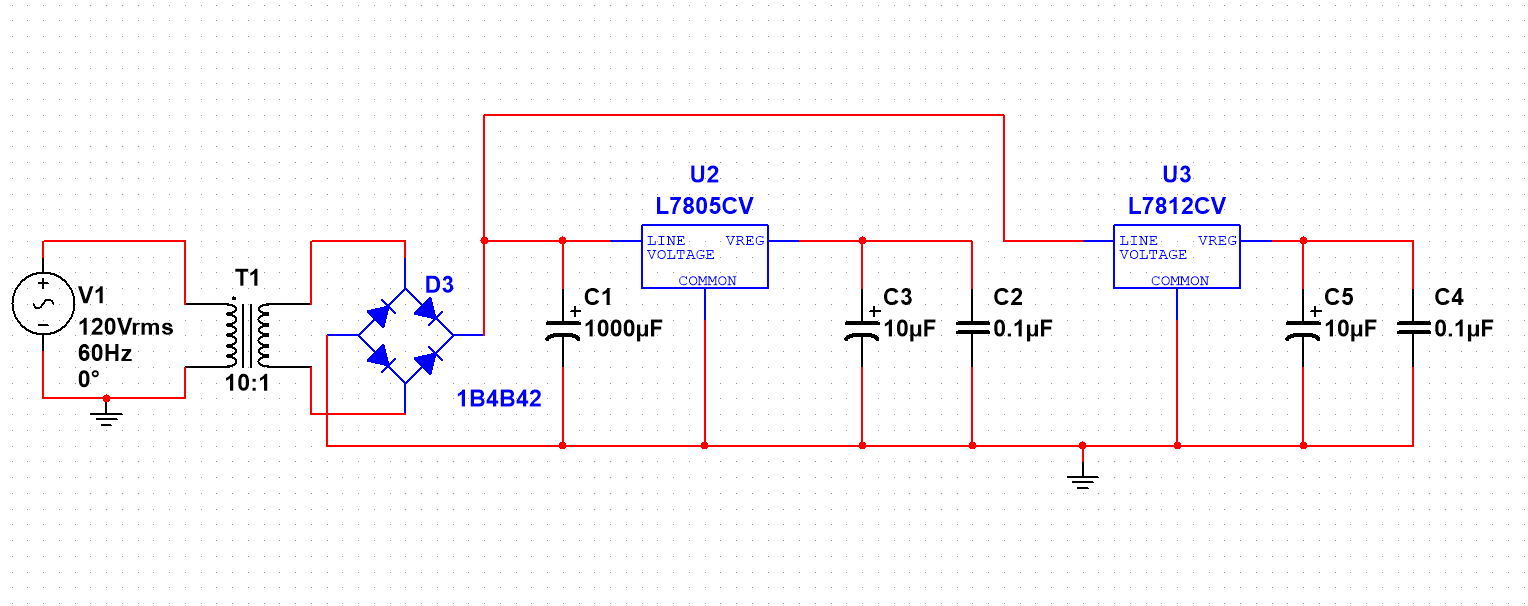
\includegraphics[width=0.7\textwidth]{diagrama_alimentacion.png}
		\caption{Diagrama del circuito de Alimentación.}
		\label{fig:alimentacion}
	\end{figure}
	
	\subsection{Justificación de diseño}
	El diseño del circuito de alimentación de la Fig. \ref{fig:alimentacion} se fundamenta en la necesidad de convertir los 120\,$\text{V}_{\text{rms}}$ de corriente alterna (CA) a voltajes de corriente directa (CD) regulados estables, habitualmente de 5\,V para los componentes de lógica digital (TTL/CMOS), y otros voltajes mayores (como 12\,V) si así lo requieren la amplificación de la señal acústica o los arreglos de LEDs de alta luminosidad.\\
	
	Inicialmente, el transformador reductor disminuye el voltaje de entrada a un nivel seguro y apto para su manipulación. Luego, el puente rectificador de diodos convierte la señal alterna en una señal pulsante en una sola dirección. Para disminuir el rizado de esta señal, se incorporan capacitores de gran valor en capacitancia que filtran las oscilaciones y otorgan una primera etapa de estabilización a la señal.\\
	
	Finalmente, los reguladores de voltaje integrados (como los de la familia 78XX) proporcionan una salida continua y fija, absorbiendo las variaciones en el consumo de corriente al encender diferentes estados del semáforo. Se agregan capacitores de desacople adicionales en los terminales de entrada y salida de estos reguladores para estabilizar la respuesta transitoria del dispositivo y atenuar posibles ruidos de alta frecuencia introducidos por la conmutación lógica, garantizando así un desempeño ininterrumpido en todo el circuito de control de tráfico.\\

\newpage

\section{\textbf{Máquina de estados}}
\subsection{Descripción}
Esta subsección describe el circuito encargado de controlar la lógica completa del semáforo vehicular y peatonal, incluyendo la generación de estados, temporización, control de transición y activación de las señales luminosas. El circuito implementa una máquina de estados síncrona basada en lógica digital discreta, utilizando compuertas lógicas, contadores y temporizadores,
cumpliendo con las especificaciones establecidas para el proyecto de semáforo vehicular y peatonal.
La FSM consta de cuatro estados codificados mediante dos bits, los cuales son almacenados en dos flip-flops JK CD4027 sincronizados por una señal de reloj generada con un temporizador 555. Cada estado representa una etapa específica del funcionamiento del semáforo peatonal y vehicular, permitiendo controlar tanto las luces como las señales sonoras del sistema.
 \\

\subsection{Diagrama de la FSM}
	% Descomente y ajuste el nombre de la imagen:
	
	\begin{figure}[H]
		\centering
		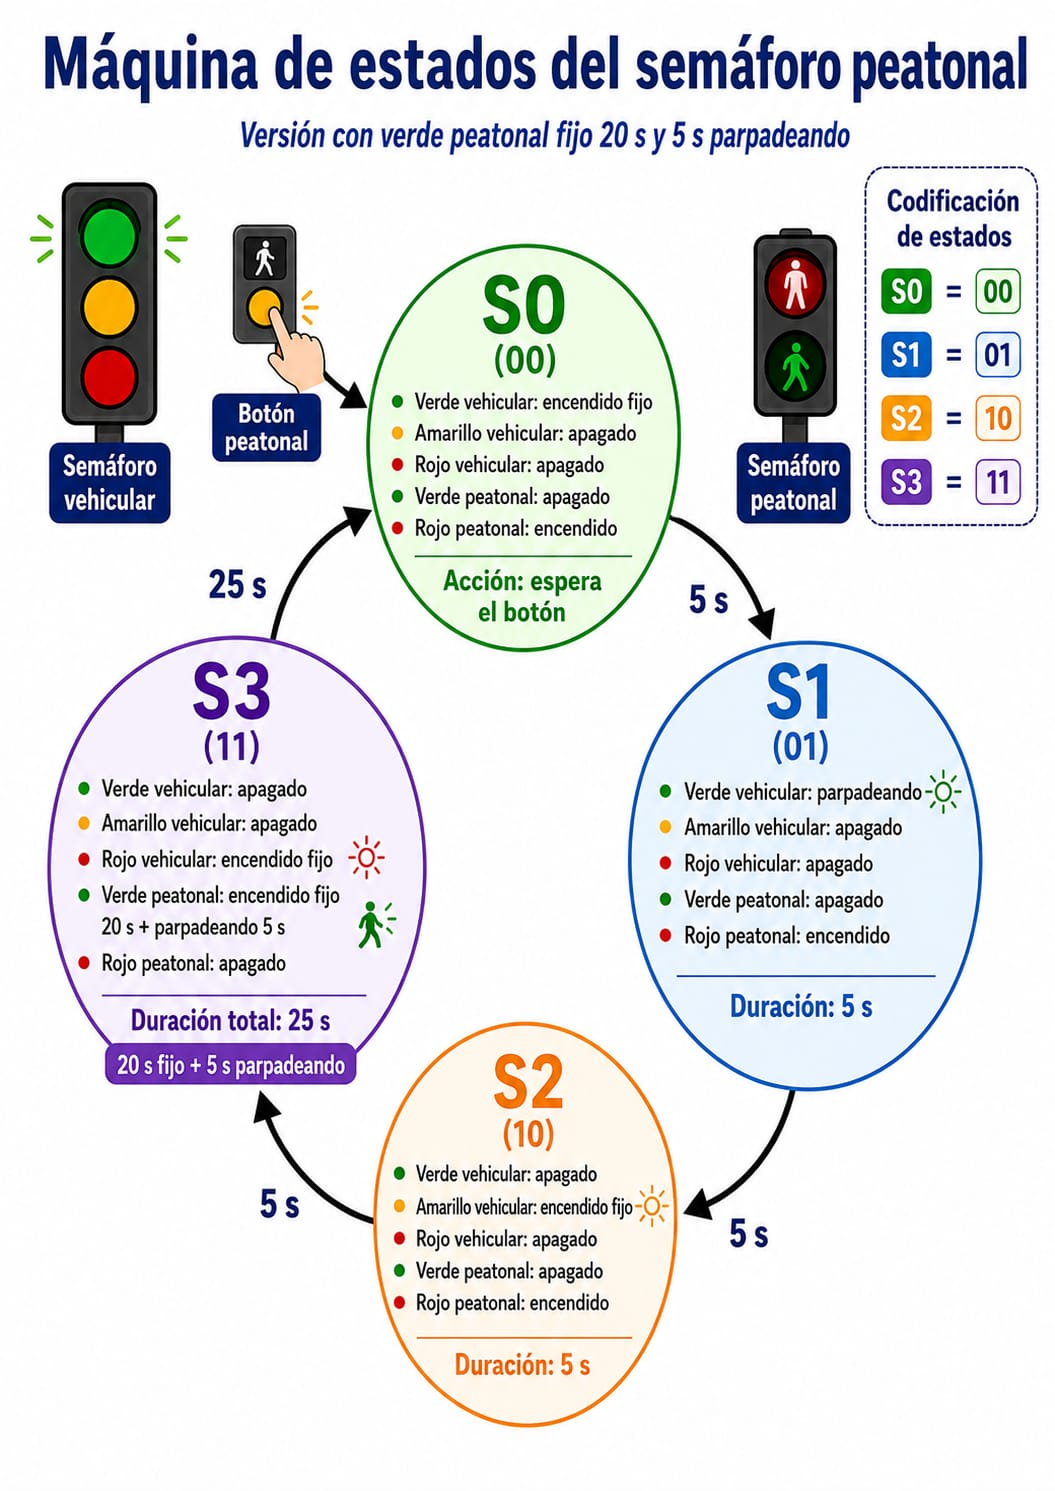
\includegraphics[width=0.6\textwidth]{Diagrama_de_FSM.jpeg}
		\caption{Diagrama del flujo de la máquina de estados.}
		\label{_diagrama_fsm}
	\end{figure}

El estado inicial del sistema es $S_0 (00)$. En este estado el semáforo vehicular permanece en verde fijo, mientras que el semáforo peatonal se mantiene en rojo. Esta condición representa el funcionamiento normal del cruce cuando no existe una solicitud peatonal. La máquina permanece indefinidamente en $S_0$ hasta que se presiona el botón peatonal. Al detectarse esta solicitud, el circuito fuerza la transición hacia $S_1$, iniciando la secuencia de cambio de luces.\\

En $S_1 (01)$, el verde vehicular comienza a parpadear durante 5 segundos. Esta etapa cumple la función de advertir a los conductores que el paso vehicular está próximo a finalizar. Durante este estado, el semáforo peatonal continúa en rojo, por lo que el peatón aún no tiene permitido cruzar.\\

Luego, la FSM avanza hacia $S_2 (10)$, donde se enciende el amarillo vehicular de forma fija durante 5 segundos. Este estado funciona como etapa de transición entre el paso vehicular y el paso peatonal, permitiendo que los vehículos despejen la intersección antes de que se active el rojo vehicular.\\

Posteriormente, el sistema entra en $S_3 (11)$. En este estado se apaga el verde y el amarillo vehicular, se enciende el rojo vehicular y se habilita el verde peatonal. La duración total de $S_3$ es de 25 segundos. Durante los primeros 20 segundos, el verde peatonal permanece encendido de forma fija, indicando que el cruce está permitido. Durante los últimos 5 segundos, el verde peatonal comienza a parpadear, advirtiendo al peatón que el tiempo de cruce está por finalizar. Al cumplirse el tiempo total de $S_3$, la máquina retorna automáticamente al estado $S_0$.\\

Para controlar la temporización de $S_3$ se emplea un contador CD4017. Este contador permite dividir el estado peatonal en intervalos de 5 segundos. La señal L5 se toma de la salida Q4 del CD4017, ya que esta salida se activa durante los últimos 5 segundos del estado $S_3$. Por lo tanto, L5 se utiliza para dos funciones principales: activar el parpadeo del verde peatonal en la etapa final del cruce y permitir el retorno de la máquina al estado S0 una vez concluido el tiempo peatonal.\\

Además, el circuito utiliza una señal de parpadeo denominada BLINK, generada mediante una señal de reloj de 1 Hz. Esta señal se combina con la lógica de estados para hacer parpadear el verde vehicular durante S1 y el verde peatonal durante los últimos 5 segundos de $S_3$.\\

\subsection{Diagrama de la FSM}
	% Descomente y ajuste el nombre de la imagen:
	
	\begin{figure}[H]
		\centering
		
\includegraphics[width=1\textwidth]{Diagrama_Multisim_FSM.jpg}
		\caption{Diagrama del flujo de la máquina de estados.}
		\label{fsm1}
	\end{figure}
	
	
\subsection{Justificación de diseño}

La implementación de la máquina de estados se realizó utilizando un \textit{clock}, debido a que este tipo de arquitectura permite controlar de forma ordenada la secuencia de eventos del semáforo, garantizando que cada transición ocurra únicamente cuando se cumplen las condiciones establecidas y evitando cambios indeseados en las salidas.

\begin{itemize}
    \item \textbf{Temporizador 555:} Se seleccionó un temporizador 555 configurado en modo astable para generar la señal de reloj del sistema, debido a su precisión para controlar las transiciones temporizadas de la máquina de estados.\\

    \item \textbf{Flip-flops JK CD4027:} Se emplearon dos flip-flops JK debido a que con ellos es posible almacenar los dos bits que representan los cuatro estados de funcionamiento del sistema.\\

    \item \textbf{Lógica combinacional:} La lógica combinacional se diseñó para generar tanto las ecuaciones de próximo estado como las señales de salida respectivas de cada estado. Esta implementación permite controlar de manera simultánea el encendido de los semáforos vehiculares y peatonales, la activación del sistema sonoro y las señales de control requeridas por el resto del circuito.\\

    \item \textbf{Contador CD4017:} Se utilizó un contador decimal CD4017 para controlar la duración de cada estado mediante la generación de pulsos de reloj provenientes del temporizador 555. Las salidas del contador se emplean para habilitar las transiciones entre estados y sincronizar el funcionamiento de los displays de siete segmentos.\\

    \item \textbf{LEDs transistorizados:} Aunque la lógica CMOS es capaz de suministrar corriente limitada, se utilizaron transistores BJT como interruptores para accionar los LED de los semáforos. Esto evita sobrecargar las salidas de los circuitos integrados y permite alimentar los indicadores directamente desde la fuente de $5\,\mathrm{V}$ sin afectar el funcionamiento de la lógica digital.\\
\end{itemize}

\newpage

\section{\textbf{Display 7-Segmentos}}
\subsection{Descripción}
El módulo de display fue diseñado para implementar el conteo regresivo visual del sistema de semáforo vehicular y peatonal. Su función principal consiste en mostrar al usuario el tiempo restante disponible durante la habilitación del paso peatonal.\\

El sistema utiliza un temporizador 555 en configuración astable como generador de pulsos de reloj, encargado de producir la señal periódica que sincroniza el conteo. Esta señal es enviada a dos contadores BCD CD4510, uno destinado al manejo de las unidades y otro al de las decenas del conteo regresivo.\\

Las salidas BCD de cada contador son conectadas a decodificadores CD4511, los Las salidas BCD de cada contador son conectadas a decodificadores CD4511, los cuales convierten la información binaria en las señales necesarias para controlar los displays de 7 segmentos. Además, cada segmento incorpora una resistencia limitadora de corriente de 330\,$\Omega$ con el objetivo de proteger tanto los displays como los circuitos integrados.\\

El módulo fue configurado para iniciar el conteo en 20 segundos, disminuyendo progresivamente hasta llegar a 00, permitiendo visualizar el tiempo restante para el cruce peatonal. Además, se implementará una lógica de detección de cero mediante compuertas lógicas, de manera que cuando el sistema detecta simultáneamente 00 en decenas y unidades, el reloj queda bloqueado y el contador deja de disminuir, evitando conteos inválidos posteriores al cero.


\subsection{Diagrama del circuito}
	% Descomente y ajuste el nombre de la imagen:
	
	\begin{figure}[H]
		\centering
		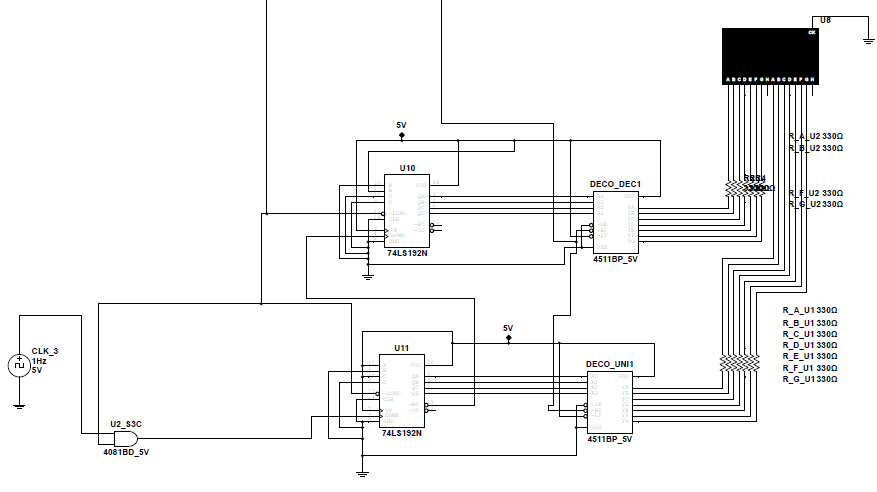
\includegraphics[width=0.9\textwidth]{Diagrama_Multisim_Display.png}
		\caption{Diagrama del circuito del Display de 7-segmentos en el software Multisim.}
		\label{diag_circuito_display}
	\end{figure}
		
	
\subsection{Justificación de diseño}
El diseño del módulo de display se desarrolló utilizando componentes digitales discretos debido a la necesidad de implementar un sistema de conteo regresivo confiable, visible y compatible con la lógica general del semáforo peatonal. Se seleccionaron contadores BCD CD4510 porque permiten realizar conteos descendentes de manera sencilla y facilitan la manipulación de valores decimales sin requerir lógica adicional compleja.\\

Asimismo, se emplearon decodificadores CD4511 debido a su compatibilidad directa con displays de 7 segmentos de cátodo común, reduciendo significativamente la cantidad de conexiones y simplificando la implementación física del sistema. Esto permite obtener una visualización clara del tiempo restante para el cruce peatonal.\\

La utilización del temporizador 555 como generador de reloj se debe a su facilidad de configuración, estabilidad y bajo costo, permitiendo generar pulsos periódicos necesarios para sincronizar el conteo del sistema. Además, las resistencias limitadoras fueron incorporadas para proteger los segmentos LED de sobrecorrientes y aumentar la confiabilidad del circuito.\\

Finalmente, de esta manera se puede verificar individualmente que este bloque sea funcional antes de integrar el sistema completo del semáforo.\\


\begin{figure}[H]
		\centering
		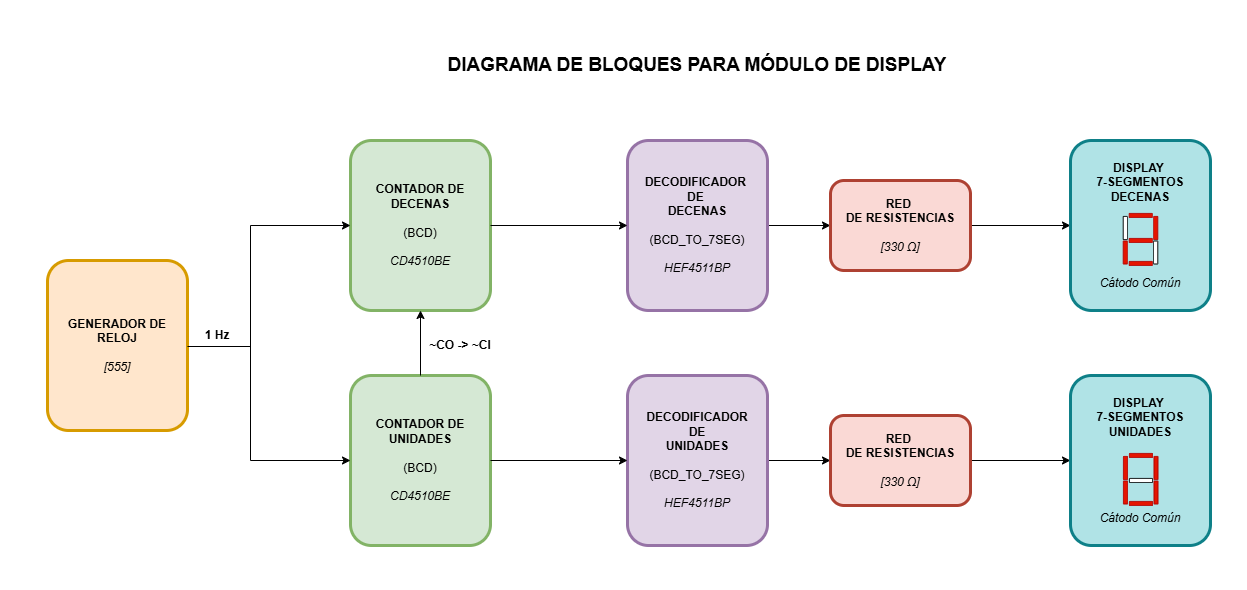
\includegraphics[width=1\textwidth]{Diagrama_de_bloques_Display.png}
		\caption{Diagrama de bloques para el Display.}
		\label{diag_bloq_display}
	\end{figure}
	
\newpage
	
\section{\textbf{Sistema de Señalización Auditiva}}

\subsection{Descripción}

Este sistema fue diseñado con el propósito de generar una señal auditiva para los peatones cuando esté permitido cruzar la calle. Consiste en generar un sonido periódico cuando el semáforo peatonal se encuentre en verde, y que este mismo se acelere una vez que falten cinco segundos para que vuelva a ponerse en rojo.\\

Tomando en cuenta las especificaciones solicitadas, cumpliendo únicamente con el uso de electrónica básica y sin ningún tipo de microcontroladores, se llegó a la conclusión de que la mejor forma de manejarlo era por medio de osciladores astables con circuitos integrados 555, los cuales permiten ajustar la frecuencia deseada mediante resistencias y capacitores.\\

Dados estos requerimientos, el sistema completo se divide en los siguientes bloques funcionales principales:

\begin{enumerate}
    \item Generación del tono audible.
    \item Generación de la frecuencia de repetición lenta.
    \item Generación de la frecuencia de repetición rápida.
    \item Etapa de selección y amplificación de potencia.
\end{enumerate}

En cuanto al funcionamiento del circuito, todo inicia con la generación de tres señales cuadradas mediante temporizadores 555 configurados como osciladores astables. La primera corresponde al tono audible, con una frecuencia aproximada de $1\,\mathrm{kHz}$, seleccionada por encontrarse dentro del rango de mayor sensibilidad del oído humano y, por tanto, ser fácilmente perceptible. Adicionalmente, se generan dos señales de aproximadamente $1\,\mathrm{Hz}$ y $2\,\mathrm{Hz}$, las cuales se emplean para producir las velocidades de repetición lenta y rápida del tono, respectivamente.\\

Posteriormente, la selección de la velocidad y la habilitación del sonido se realizan mediante un multiplexor (MUX). Este recibe como señales de control las salidas provenientes de la máquina de estados, específicamente las señales \texttt{PEATONAL\_ROJO} y \texttt{ULTIMOS\_5\_SEG}. Dependiendo de la combinación de estas entradas, el multiplexor selecciona una de las tres posibles salidas: ausencia de sonido, repetición lenta ($1\,\mathrm{Hz}$) o repetición rápida ($2\,\mathrm{Hz}$). De esta manera, se concentra en un único bloque la lógica necesaria para determinar el comportamiento del sistema de audio según el estado del semáforo. La señal de salida habilitada por el multiplexor se combina finalmente mediante una compuerta AND con el tono audible de $1\,\mathrm{kHz}$.\\

Para la etapa de amplificación, dado que la lógica digital entrega una amplitud de $5\,\mathrm{V}$ pero con una capacidad de corriente baja para el uso requerido, se implementa inicialmente un divisor de tensión para adaptar el nivel de entrada del amplificador. Posteriormente, la señal atraviesa un amplificador de dos etapas: una primera etapa de ganancia de voltaje basada en un transistor en configuración de emisor común y una segunda etapa de potencia tipo \textit{push-pull} clase AB, ambas alimentadas con una fuente de $12\,\mathrm{V}$. Esta configuración proporciona tanto la ganancia de tensión como la capacidad de corriente necesarias para accionar el parlante de forma adecuada, garantizando un nivel de sonido adecuado para la aplicación.\\

\subsection{Diagrama del circuito}

	\begin{figure}[H]
		\centering
		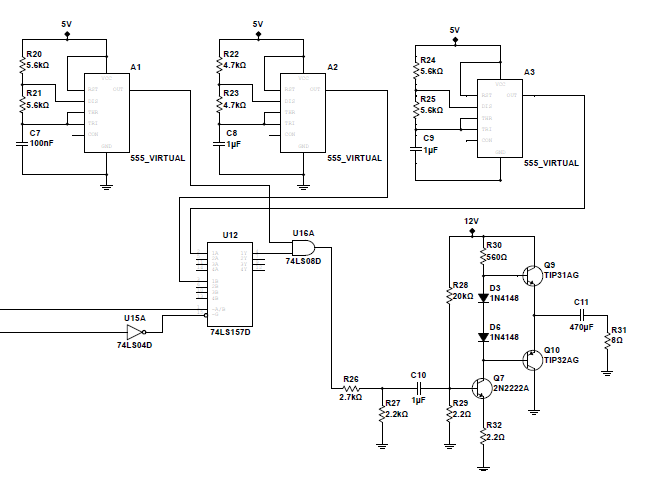
\includegraphics[width=0.7\textwidth]{circ audio.png}
		\caption{Diagrama del circuito de señalización auditiva.}
		\label{audio}
	\end{figure}

\subsection{Justificación de Diseño}

En esta sección se justifica la selección de los principales componentes utilizados en la implementación del circuito de generación y amplificación del tono audible.\\

\begin{itemize}
    \item \textbf{Temporizadores 555:} Se emplearon tres temporizadores 555 configurados en modo astable debido a su simplicidad y estabilidad para generar señales cuadradas. Un primer temporizador produce el tono audible de aproximadamente $1\,\mathrm{kHz}$, mientras que los otros dos generan las frecuencias de repetición de $1\,\mathrm{Hz}$ y $2\,\mathrm{Hz}$, correspondientes a las velocidades lenta y rápida requeridas. Además, estos circuitos integrados permiten ajustar fácilmente la frecuencia mediante la selección de resistencias y capacitores.\\

    \item \textbf{Multiplexor:} Se seleccionó un multiplexor como bloque de decisión debido a que simplifica considerablemente la lógica de selección de la señal de salida. A partir de las señales de control \texttt{PEATONAL\_ROJO} y \texttt{ULTIMOS\_5\_SEG}, el MUX determina automáticamente si la salida debe permanecer deshabilitada o si debe haber una repetición lenta o rápida. Esta solución reduce la cantidad de compuertas lógicas necesarias.\\

    \item \textbf{Compuerta AND:} La salida del multiplexor se combina mediante una compuerta AND con la señal de $1\,\mathrm{kHz}$. De esta manera, el tono audible únicamente está presente cuando la señal de habilitación seleccionada por el MUX se encuentra activa.\\

    \item \textbf{Divisor de tensión:} Antes de la etapa de amplificación se implementó un divisor de tensión para adaptar el nivel de la señal proveniente de la lógica digital al valor requerido por la etapa amplificadora. Esto permite establecer un punto de operación adecuado para el transistor de entrada.\\

    \item \textbf{Amplificador en emisor común:} La primera etapa de amplificación corresponde a un amplificador de voltaje con transistor BJT en configuración de emisor común. Esta topología fue elegida por su elevada ganancia de voltaje y su facilidad de diseño.\\

    \item \textbf{Etapa \textit{push-pull} clase AB:} Como etapa final se implementó un amplificador de potencia \textit{push-pull} clase AB alimentado con $12\,\mathrm{V}$. Esta configuración proporciona la corriente necesaria para activar adecuadamente el parlante. Se debe tomar en cuenta que, por la corriente manejada, se utilizaron transistores de potencia mucho más robustos y con alta capacidad de disipación de calor.\\

    \item \textbf{Parlante:} Se utilizó un parlante para convertir la señal eléctrica amplificada en una señal sonora. La selección de un amplificador de potencia previo garantiza que el parlante reciba la corriente suficiente para producir un nivel de sonido adecuado para la aplicación.\\
\end{itemize}

\newpage
	
\section{Implementación del circuito en protoboard}

Una vez verificado el funcionamiento de cada uno de los módulos de forma individual, se procedió a la integración del sistema completo sobre protoboard. La implementación se realizó distribuyendo los bloques funcionales de manera independiente para facilitar el proceso de análisis e integración. Cada módulo fue conectado a la fuente de alimentación correspondiente, asegurando que los niveles de tensión requeridos fueran suministrados de manera estable y confiable.

\subsection{Integración del sistema}

Una vez verificado el funcionamiento individual de cada uno de los módulos, se procedió a su integración para conformar el sistema completo. La FSM es el bloque central del circuito, ya que a partir de sus salidas se generan todas las señales de control necesarias para coordinar el funcionamiento del resto de los módulos.

Las señales correspondientes a los estados de la FSM se distribuyen tanto al circuito de señalización visual como al circuito de generación de sonido. En el módulo de displays de siete segmentos, estas señales habilitan la carga y el funcionamiento de los contadores, permitiendo que el conteo regresivo esté enlazado con el estado del cruce peatonal.

De forma paralela, las señales \texttt{PEATONAL\_ROJO} y \texttt{ULTIMOS\_5\_SEG} son enviadas al circuito de audio, donde controlan el multiplexor encargado de seleccionar la velocidad del tono audible. Posteriormente, la señal seleccionada se combina con el tono de $1\,\mathrm{kHz}$ y es enviada a la etapa amplificadora, la cual suministra la potencia necesaria para el parlante.

Asimismo, las salidas de la máquina de estados controlan mediante lógica combinacional las etapas de conmutación de los LED correspondientes a los semáforos.

Todos los módulos comparten una referencia común de tierra y la lógica del sistema, incluyendo los circuitos integrados CMOS, TTL, los displays y los LED, opera con una alimentación de $5\,\mathrm{V}$, mientras que la etapa de potencia del amplificador utiliza una fuente independiente de $12\,\mathrm{V}$.

\subsection{Montaje del protoboard}

La Figura~\ref{fig:montaje-protoboard} muestra el montaje final del sistema sobre protoboard. La distribución de los módulos se realizó de forma que facilitara tanto la interconexión entre ellos como las labores de prueba y depuración durante la etapa de implementación.

En el extremo derecho del montaje se ubica la fuente de alimentación, desde donde se distribuyen los niveles de tensión requeridos por los diferentes módulos del sistema. En la región central se implementó la máquina de estados finitos junto con la lógica de control, la cual constituye el núcleo del proyecto al generar las señales que coordinan el funcionamiento del resto de los bloques.

En la parte inferior del protoboard se localiza el módulo de señalización visual, conformado por los contadores, los decodificadores y los displays de siete segmentos encargados de mostrar el tiempo restante del cruce peatonal. Finalmente, en el lado izquierdo se encuentra el circuito de generación y amplificación de audio, incluyendo la lógica de selección de la cadencia del tono, el generador de la señal audible y la etapa amplificadora encargada de alimentar el parlante.

\begin{figure}[H]
    \centering
    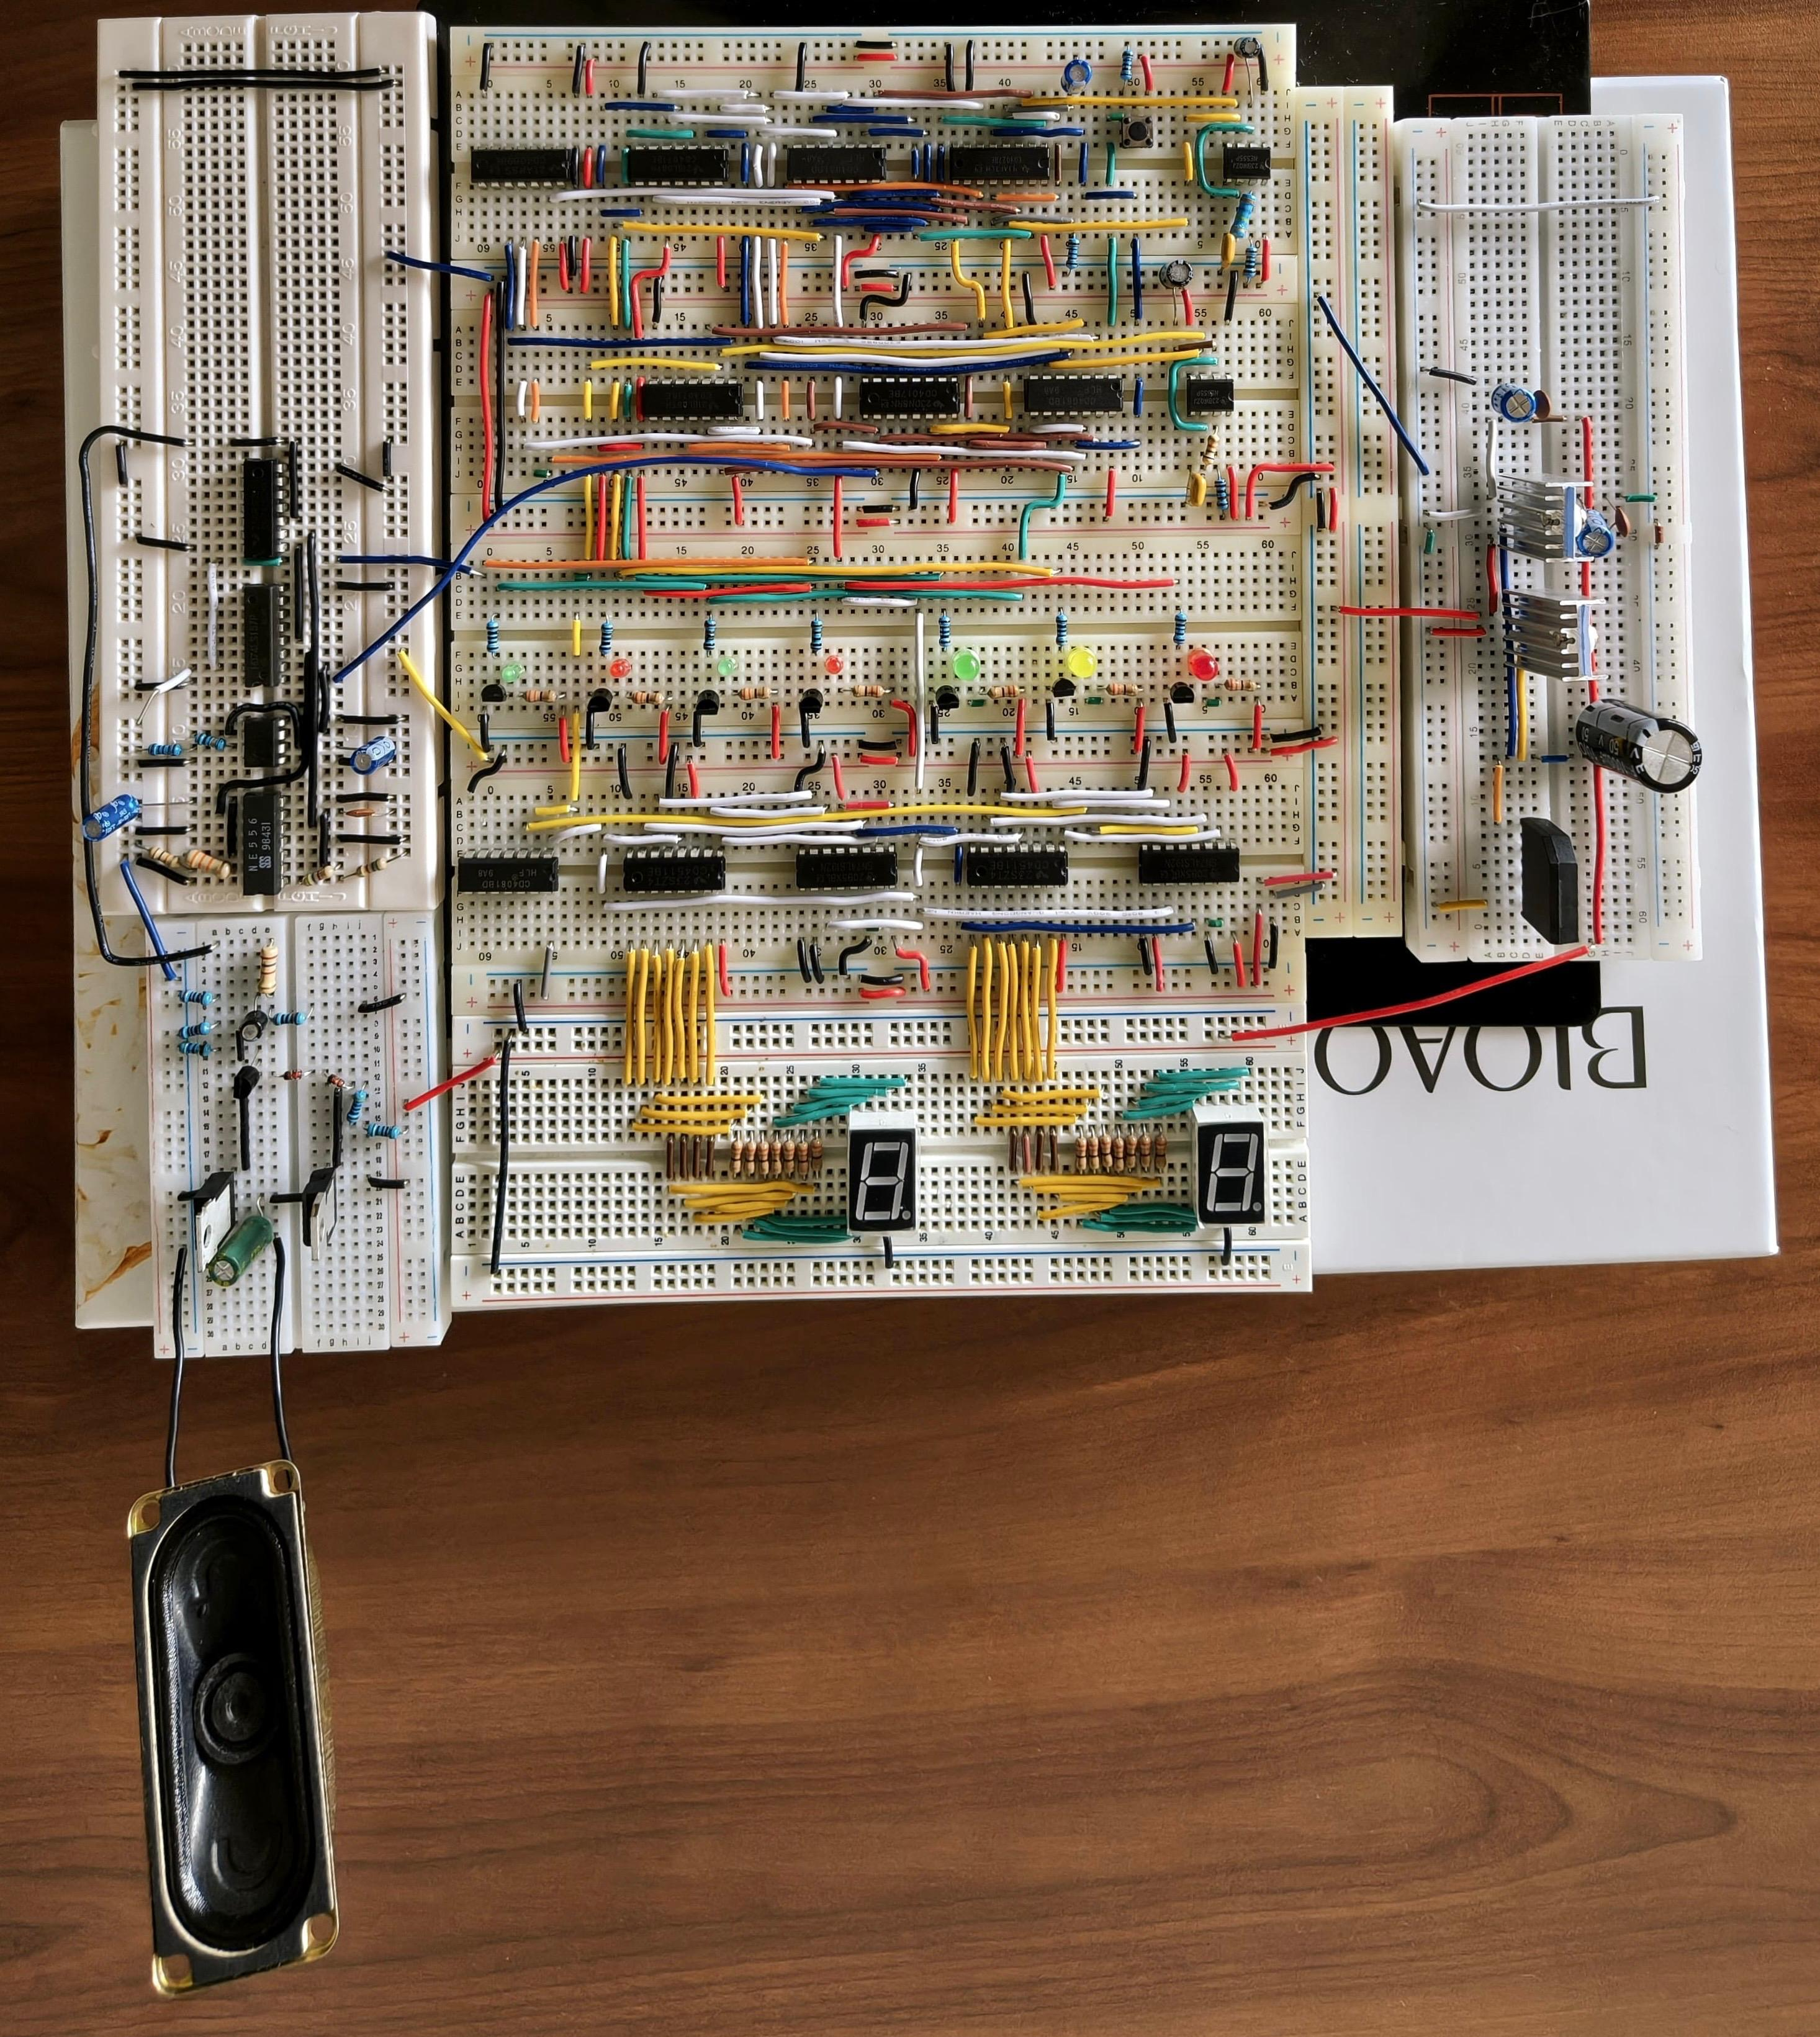
\includegraphics[width=0.9\linewidth]{circ proto.jpeg}
    \caption{Circuito completo implementado en protoboard.}
    \label{fig:montaje-protoboard}
\end{figure}

\newpage

\section{Diseño de la PCB}

Con el objetivo de introducir el proceso de diseño PCBs, se decidió implementar la fuente de alimentación del sistema sobre una placa independiente. Este módulo fue seleccionado debido a su menor complejidad en comparación con el resto de sistemas, permitiendo familiarizarse con las herramientas de diseño.\\

Durante el diseño se buscó obtener una distribución compacta de los componentes, procurando aprovechar el área disponible sin generar un montaje excesivamente denso que dificultara el diseño. Asimismo, se mantuvo una separación adecuada entre los componentes para facilitar tanto la soldadura.\\

Para simplificar la conexión de la fuente con el resto del sistema, se incorporaron borneras de dos terminales tanto en la entrada como en la salida de la placa. Estas permiten realizar las conexiones con cables más cómodamente.\\

El enrutamiento de las pistas se realizó procurando minimizar cruces innecesarios y mantener recorridos lo más cortos posible, contribuyendo a un diseño ordenado y de fácil fabricación.\\

La Figura~\ref{fig:pcb-fuente} muestra el diseño final de la tarjeta de circuito impreso desarrollada para la fuente de alimentación y la incorporación en físico de la placa PCB.\\

\begin{figure}[H]
    \centering

    \begin{subfigure}{0.45\linewidth}
        \centering
        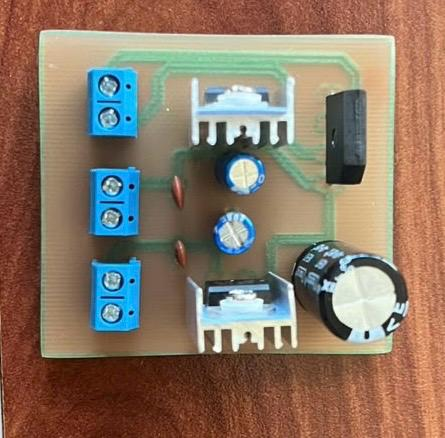
\includegraphics[width=\linewidth]{pcb.jpeg}
        \caption{Vista superior de la PCB.}
        \label{fig:pcb-fisica}
    \end{subfigure}
    \hfill
    \begin{subfigure}{0.45\linewidth}
        \centering
        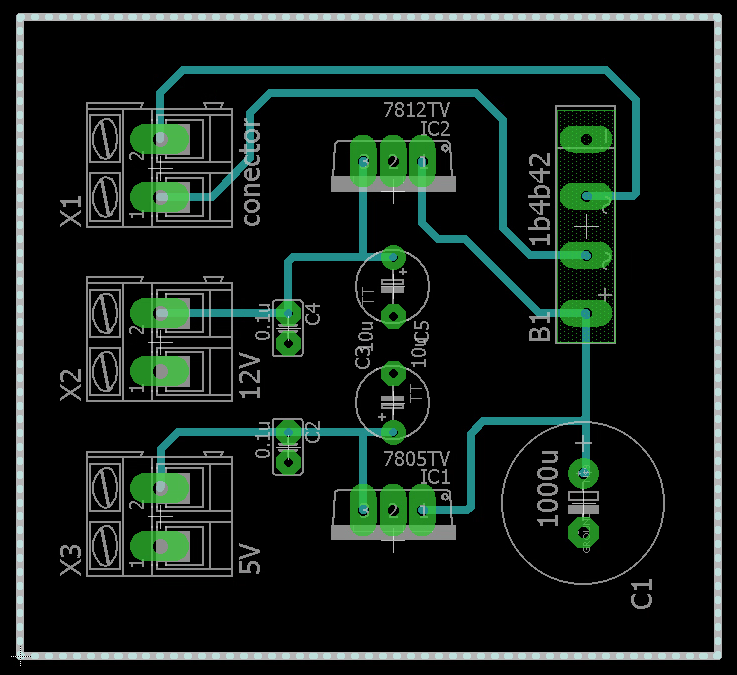
\includegraphics[width=\linewidth]{pcb_cad.png}
        \caption{Diseño de la PCB en software.}
        \label{fig:pcb-software}
    \end{subfigure}

    \caption{PCB de la fuente de alimentación.}
    \label{fig:pcb-fuente}
\end{figure}

\newpage

\section{Implementación de la maqueta}

Como complemento al desarrollo electrónico del sistema, se elaboró una maqueta física con el propósito de representar de forma visual el funcionamiento del semáforo vehicular y peatonal. Esta maqueta permite observar la aplicación del circuito en un entorno similar a un cruce real, integrando la señalización vehicular, la señalización peatonal, el botón de solicitud de cruce, los displays de conteo regresivo y el sistema de alerta auditiva.\\

La maqueta fue diseñada para facilitar la interpretación del funcionamiento del proyecto. En ella se representó una vía vehicular con su respectiva zona de paso peatonal, así como la ubicación de los semáforos correspondientes. Estos elementos se conectan directamente a las salidas de la máquina de estados, de manera que la maqueta refleja en tiempo real la secuencia lógica implementada en el circuito.\\

Desde el punto de vista constructivo, la maqueta fue elaborada utilizando materiales livianos y de fácil manipulación, como cartón,paletas, pintura y elementos decorativos. Esto permitió representar la calle, aceras, zonas verdes, señalización y otros detalles visuales que ayudan a mejorar la presentación del proyecto. La distribución de los elementos se realizó procurando que los semáforos fueran visibles y que el usuario pudiera identificar claramente el flujo de operación del sistema.\\

\subsection{Criterios de diseño de la maqueta}

Para el diseño de la maqueta se tomaron en cuenta los siguientes criterios:

\begin{itemize}
    \item \textbf{Claridad visual:} La maqueta debía permitir identificar fácilmente el semáforo vehicular, el semáforo peatonal, el paso peatonal y el botón de solicitud de cruce.

    \item \textbf{Correspondencia con el circuito:} Cada luz representada en la maqueta debía estar asociada a una salida real del circuito, de forma que el comportamiento físico coincidiera con la lógica implementada en la FSM.

    \item \textbf{Seguridad en las conexiones:} Los LED utilizados en la maqueta fueron conectados mediante resistencias limitadoras y etapas transistorizadas, evitando sobrecargar las salidas de los circuitos integrados.

    \item \textbf{Organización del cableado:} Se procuró mantener las conexiones ordenadas para facilitar la revisión del circuito, reducir errores de conexión y mejorar la presentación general del montaje.

    \item \textbf{Representación realista:} Se añadieron elementos visuales como calle, aceras, señalización y zona peatonal, con el fin de simular un entorno urbano y hacer más comprensible la función del sistema.
\end{itemize}

En general, la maqueta cumple la función de mostrar de manera práctica el resultado final del proyecto, permitiendo observar cómo la lógica electrónica controla un sistema de semáforo vehicular y peatonal completo. Además, facilita la demostración del funcionamiento ante el usuario, ya que permite visualizar las transiciones de estado, el conteo regresivo y las alertas visuales y auditivas de forma integrada.

\begin{figure}[H]
    \centering

    \begin{subfigure}{0.45\linewidth}
        \centering
        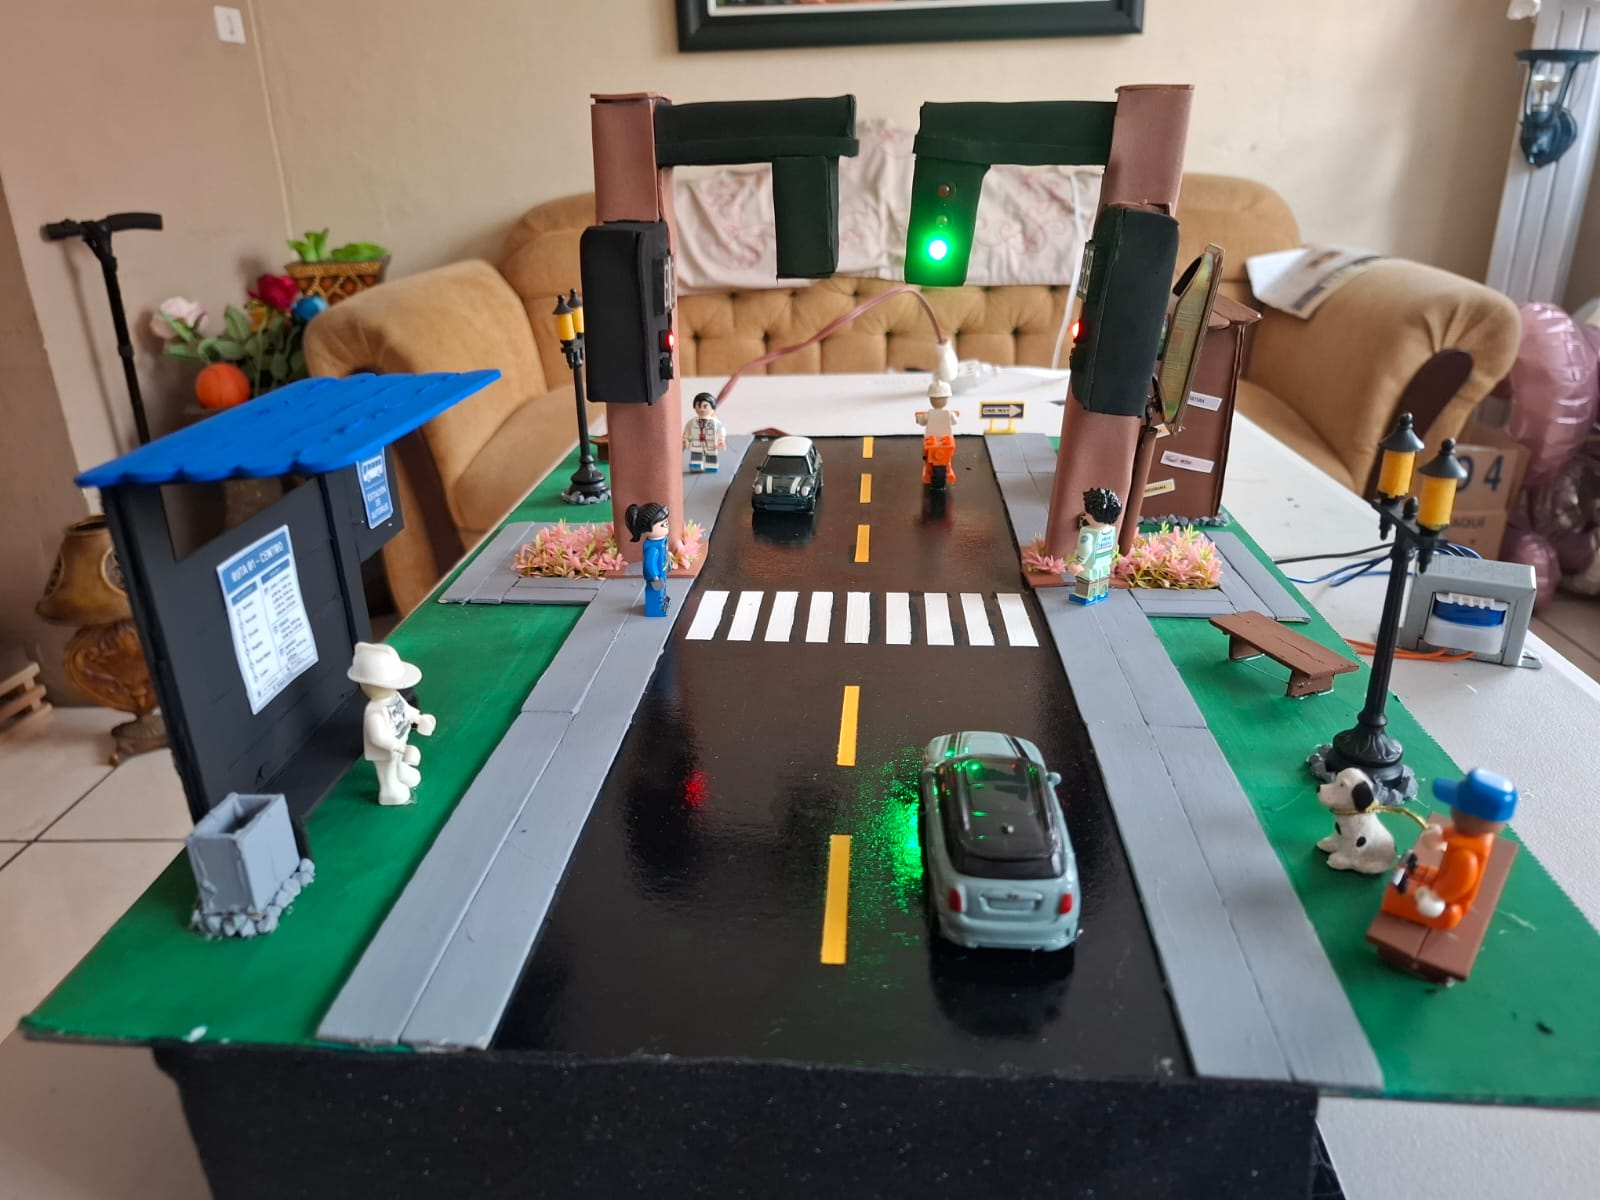
\includegraphics[width=\linewidth]{maqueta_1.jpeg}
        \caption{Vista general de la maqueta.}
        \label{fig:maqueta-1}
    \end{subfigure}
    \hfill
    \begin{subfigure}{0.45\linewidth}
        \centering
        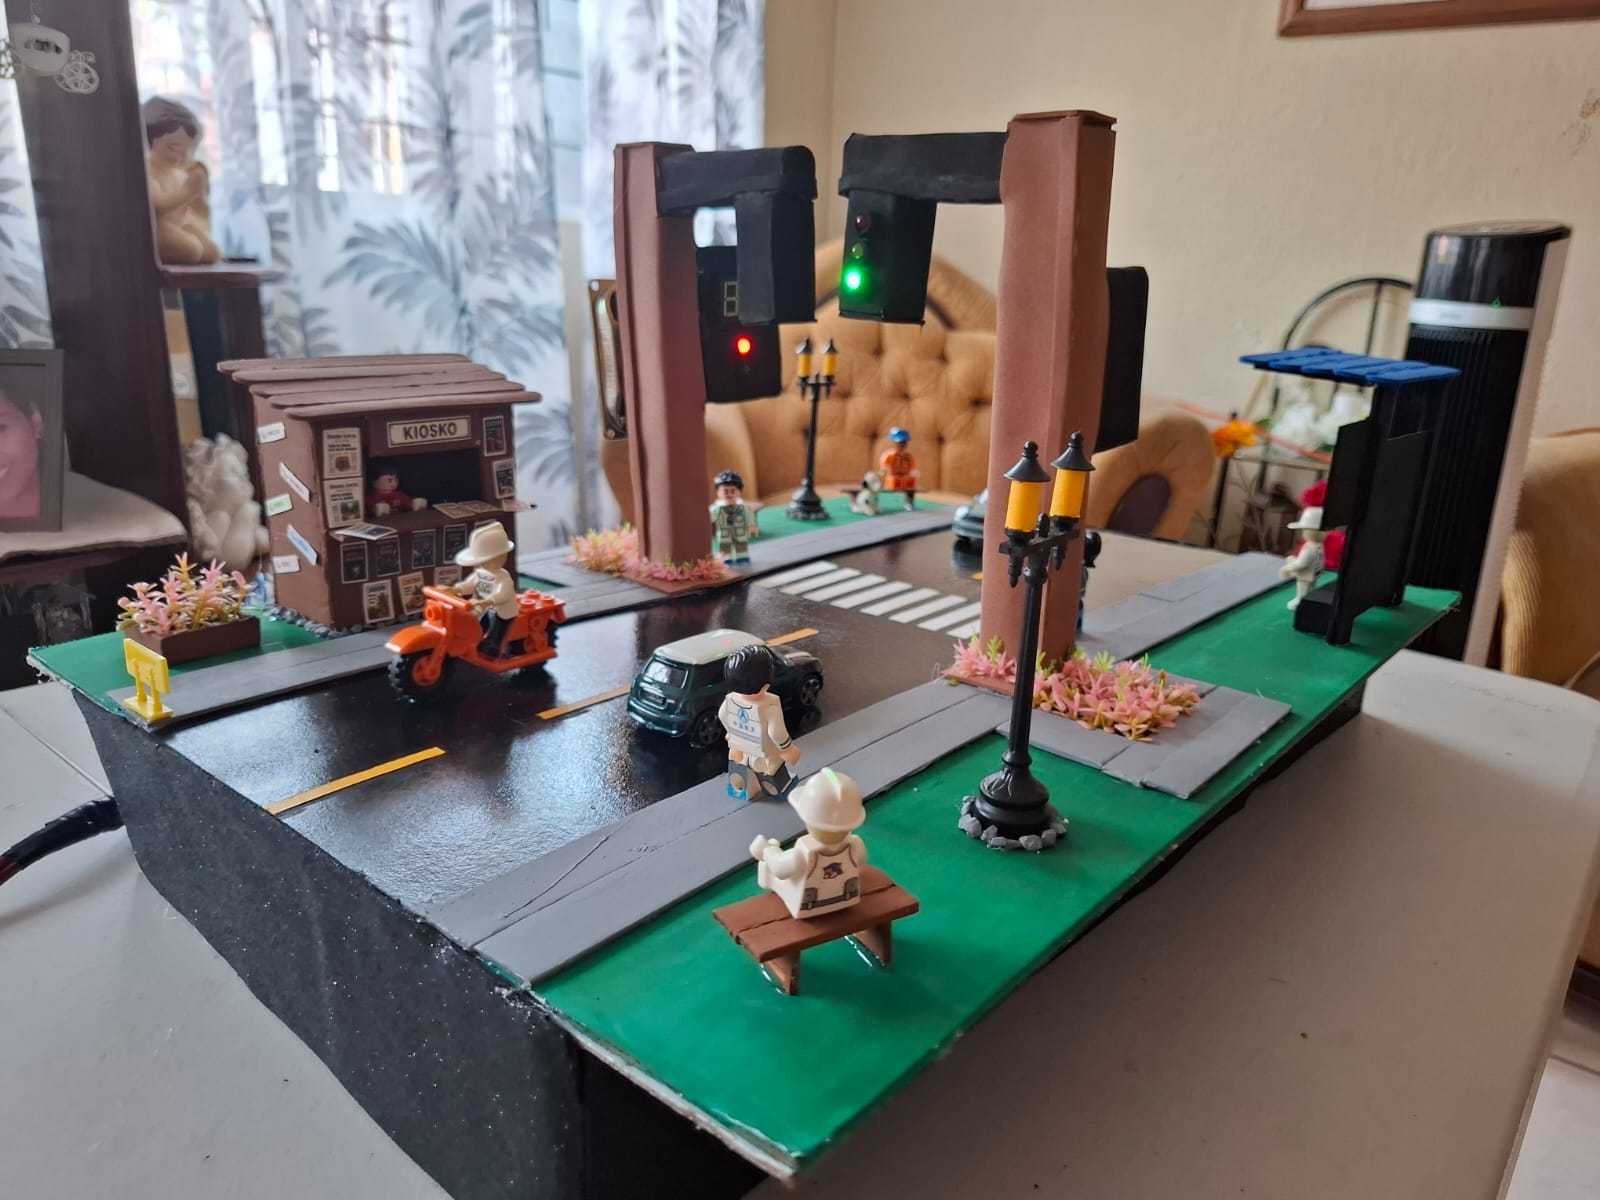
\includegraphics[width=\linewidth]{maqueta_2.jpeg}
        \caption{Vista general de la maqueta.}
        \label{fig:maqueta-2}
    \end{subfigure}

    \vspace{0.3cm}

    \vspace{0.3cm}

    \begin{subfigure}{0.45\linewidth}
        \centering
        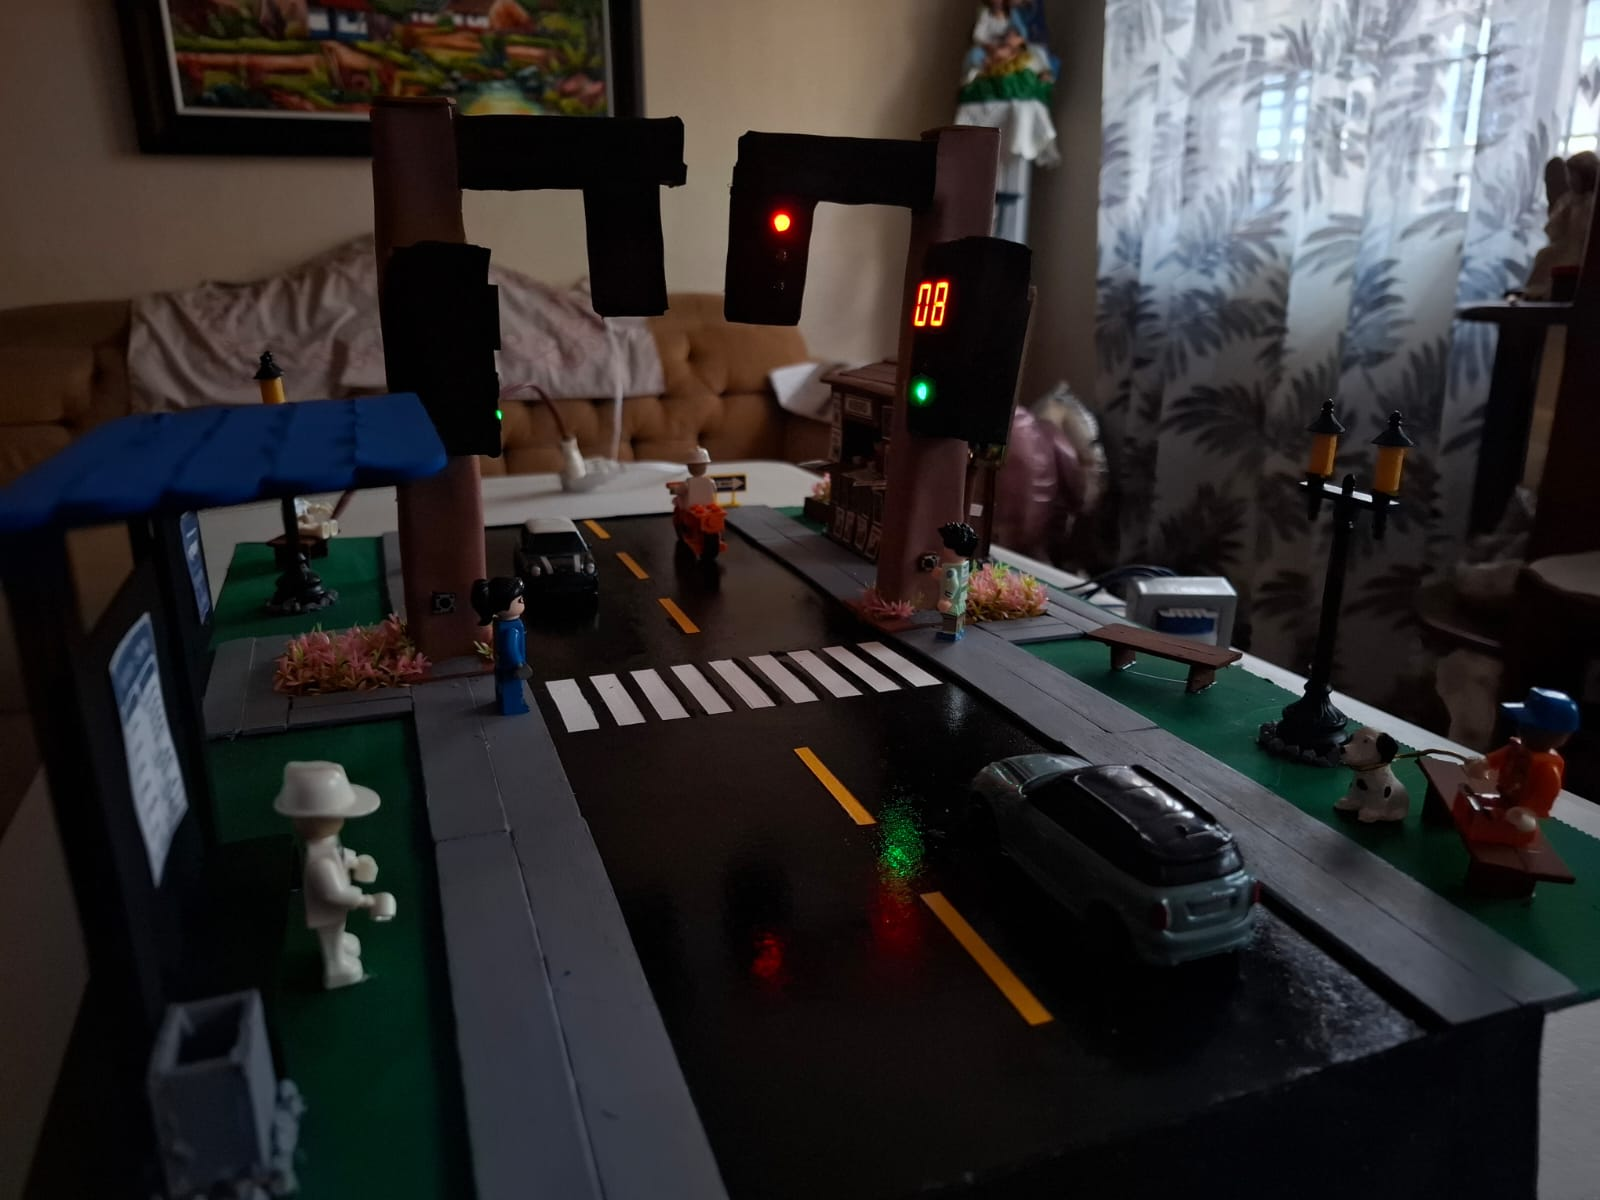
\includegraphics[width=\linewidth]{maqueta_5.jpeg}
        \caption{Muestra del estado $S_3$ en funcionamiento.}
        \label{fig:maqueta-5}
    \end{subfigure}
    \hfill
    \begin{subfigure}{0.45\linewidth}
        \centering
        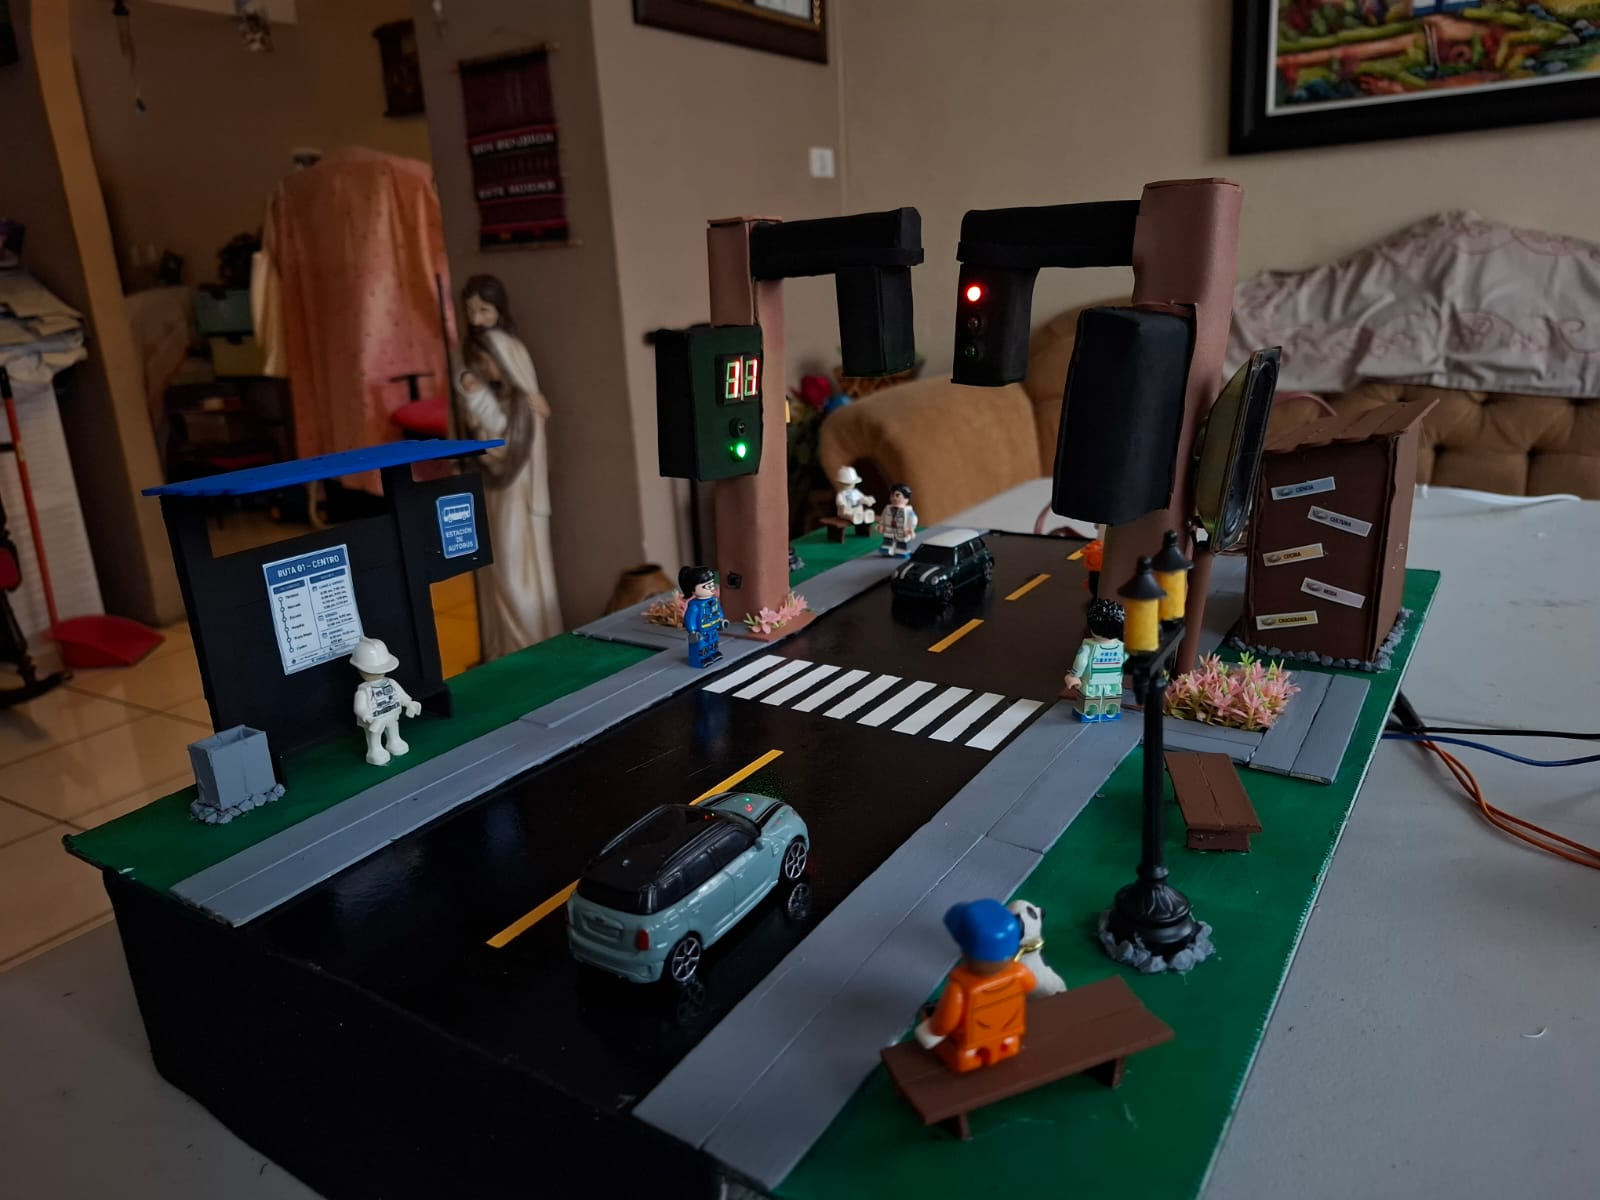
\includegraphics[width=\linewidth]{maqueta_6.jpeg}
        \caption{Muestra del estado $S_3$ en funcionamiento.}
        \label{fig:maqueta-6}
    \end{subfigure}

    \vspace{0.3cm}

    \begin{subfigure}{0.45\linewidth}
        \centering
        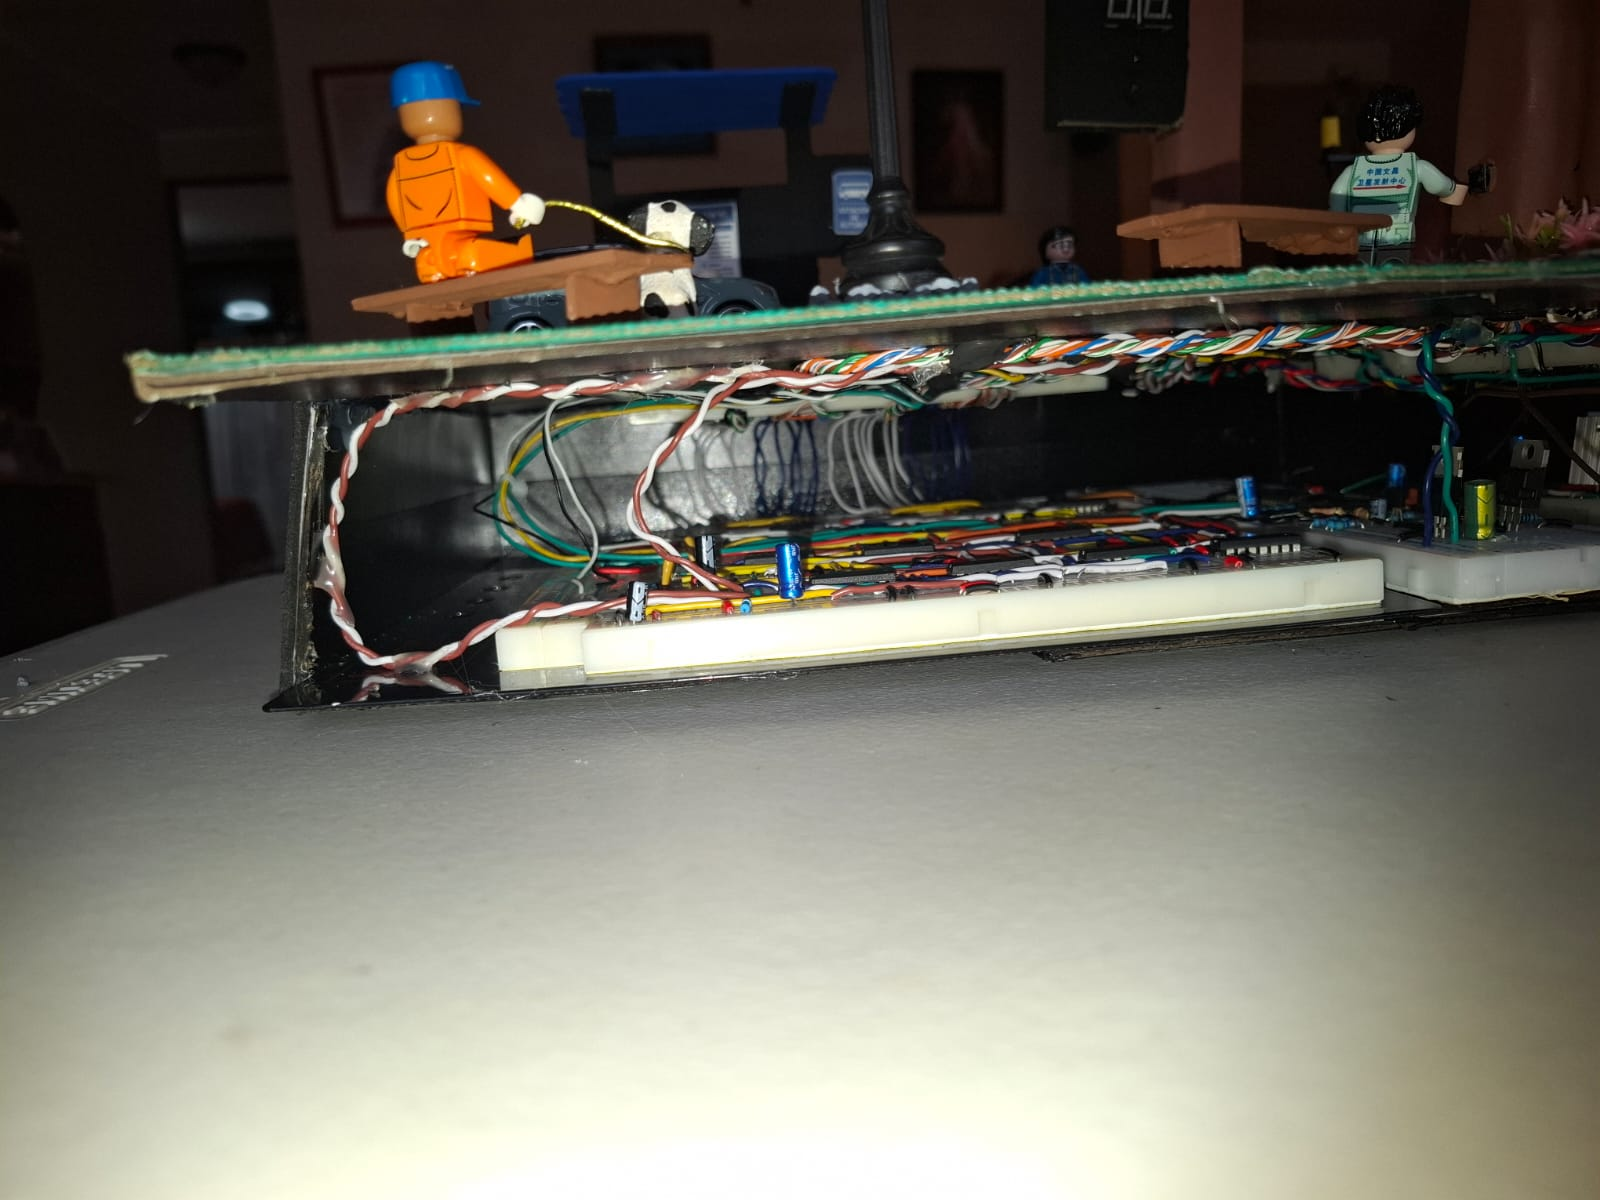
\includegraphics[width=\linewidth]{maqueta_7.jpeg}
        \caption{Integración de cableado.}
        \label{fig:maqueta-7}
    \end{subfigure}

    \caption{Mosaico de fotografías de la maqueta física del sistema de semáforo vehicular y peatonal.}
    \label{fig:mosaico-maqueta}
\end{figure}


\newpage

\section{Conclusiones}

Se logró comprobar que es completamente viable diseñar un sistema de semáforo vehicular y peatonal complejo utilizando únicamente electrónica básica y componentes discretos, cumpliendo con las especificaciones de diseño sin depender de microcontroladores programables. Esto permitió comprender con mayor profundidad la integración entre lógica digital, etapas de potencia y circuitos de control dentro de una aplicación real.\\

Se verificó que el circuito de potencia cumple con reducir y rectificar de manera segura los $120\,V_{rms}$ de la red eléctrica para entregar salidas fijas y reguladas de $5\,\mathrm{V}$ y $12\,\mathrm{V}$. Durante el diseño, se evidenció que la correcta selección de los capacitores de filtro y desacople es fundamental para reducir el rizado de la señal y absorber el ruido transitorio provocado por los constantes cambios de estado de la lógica digital.

La implementación de la máquina de estados finitos permitió coordinar la secuencia de operación del sistema, logrando que las transiciones entre las distintas fases del semáforo se realizaran de manera ordenada y sincronizada. Adicionalmente, el uso de compuertas lógicas permitió implementar el sistema de control sin requerir microcontroladores.

El sistema de señalización visual y el circuito de generación de sonido complementaron el funcionamiento del semáforo y brindan información tanto visual como auditiva al peatón. La integración de ambos módulos con la máquina de estados permitió sincronizar el conteo regresivo y la variación de la velocidad del tono audible.

Finalmente, la integración de todos los módulos sobre protoboard permitió validar el funcionamiento del sistema completo. Además, el diseño de la PCB para la fuente de alimentación sirvió como una introducción al proceso de diseño de estas tarjetas, permitiendo desarrollar criterios básicos de distribución de componentes.

\begin{thebibliography}{16}

\bibitem{floyd2008}
T. L. Floyd, \textit{Dispositivos Electrónicos}, 8.a ed. México: Pearson Prentice Hall, 2008.

\bibitem{madeincolombia555}
MADE IN COLOMBIA, ``Circuito integrado 555 explicación completa,'' YouTube, Dec. 16, 2017. [Online]. Available: \url{https://www.youtube.com/watch?v=n15R_n_TshA}

\bibitem{learning555}
``Cómo construir un circuito temporizador 555 con un retardo de apagado,'' Learning About Electronics. [Online]. Available: \url{https://www.learningaboutelectronics.com/Articulos/Circuito-temporizador-555-con-retardo-de-apagado.php}

\bibitem{electronicaled4017}
ElectronicaLED, ``Conexión y funcionamiento del circuito integrado CD4017,'' YouTube, Jun. 27, 2020. [Online]. Available: \url{https://www.youtube.com/watch?v=WflcnppydVY}

\bibitem{ic4017}
``IC 4017 Datasheet,'' ElecCircuit. [Online]. Available: \url{https://www.eleccircuit.com/ic-4017-datasheet/}

\bibitem{74ls192}
``74LS192 Decade Up/Down Counter With Clear Datasheet,'' Datasheet Hub. [Online]. Available: \url{https://www.datasheethub.com/74ls192-decade-up-down-counter-with-clear/}

\bibitem{74ls32}
``74LS32 Quad 2-Input OR Logic Gate IC Datasheet,'' Circuits DIY. [Online]. Available: \url{https://www.circuits-diy.com/74ls32-quad-2-input-or-logic-gate-ic-datasheet/}

\bibitem{74ls08}
``74LS08 Quad 2-Input AND Gate Datasheet,'' Datasheet Hub. [Online]. Available: \url{https://www.datasheethub.com/74ls08-quad-2-input-and-gate/}

\bibitem{display7seg}
``Funcionamiento del display de 7 segmentos,'' YouTube. [Online]. Available: \url{https://www.youtube.com/watch?v=892DbbZ_GYM}

\bibitem{contadoresdisplays}
``Implementación de contadores digitales y displays,'' YouTube. [Online]. Available: \url{https://www.youtube.com/watch?v=PSDCvyHsHbk}

\bibitem{maquinasestados}
``Máquinas de estados y lógica secuencial,'' YouTube. [Online]. Available: \url{https://www.youtube.com/watch?v=8t-BtlKVZ7g}

\bibitem{silva2018}
J. Silva-Martínez and E. Sánchez-Sinencio, ``Diseño e implementación de fuentes de alimentación lineales reguladas para laboratorios de electrónica,'' \textit{Revista de Educación en Ingeniería Eléctrica}, vol. 14, no. 2, pp. 45--52, Jul. 2018.

\bibitem{sadiku2021}
M. N. O. Sadiku and C. K. Alexander, \textit{Fundamentos de Circuitos Eléctricos}, 7.a ed. Ciudad de México, México: McGraw-Hill, 2021.

\bibitem{74ls14}
Renesas Technology Corp., ``HD74LS14 Hex Schmitt Trigger Inverters Datasheet,'' Rev. 3.00, Jul. 2005.

\bibitem{hef4511}
Philips Semiconductors, ``HEF4511B BCD to 7-Segment Latch/Decoder/Driver Datasheet,'' Jan. 1995.

\bibitem{ne555}
Texas Instruments, ``NA555, NE555, SA555, SE555 Precision Timers Datasheet,'' Rev. I, Sep. 2014.

\end{thebibliography}

\end{document}
